\documentclass[11pt]{article}
\usepackage[margin=1in]{geometry}
\usepackage{amsmath,amssymb}
\usepackage{graphicx}
\usepackage{booktabs}
\usepackage{xcolor}
\usepackage{listings}
\usepackage{caption}
\usepackage[colorlinks=true,linkcolor=blue!60!black,citecolor=teal!60!black,urlcolor=blue!60!black]{hyperref}
\graphicspath{{../../figures/}}

\definecolor{codebg}{gray}{0.96}
\definecolor{kw}{RGB}{0,90,160}
\definecolor{cm}{RGB}{110,120,110}
\definecolor{st}{RGB}{150,60,20}
\lstset{basicstyle=\ttfamily\footnotesize,backgroundcolor=\color{codebg},breaklines=true,
  keywordstyle=\color{kw}\bfseries,commentstyle=\color{cm}\itshape,stringstyle=\color{st},
  showstringspaces=false,frame=single,framesep=4pt,rulecolor=\color{gray!40},language=Python,
  columns=fullflexible,keepspaces=true,xleftmargin=6pt,aboveskip=6pt,belowskip=6pt}

\newcommand{\code}[1]{\texttt{\small #1}}
\title{\textbf{The Memory Meter}\\[2pt]\large A linear read-out of parametric recall for auditing\\ contamination in time-locked language models}
\author{Ranke contamination audit --- internal technical note}
\date{2026-07-10 \quad(v1.1 --- adds the orthogonalisation fix, a 278-item multi-category validation, and the meter's proper role)}

\begin{document}
\maketitle

\begin{abstract}
\noindent This note documents, at replication-grade detail, the ``memory meter'': a linear probe on a transformer's
residual stream that scores, for a single factual query, whether the model is \emph{retrieving a stored memory} or
\emph{confabulating}. We built it to audit \emph{time-locked} language models (Ranke-4B, a Qwen3-4B model frozen at a
declared knowledge cutoff) for training-data contamination---post-cutoff facts the model should not know but does. We
give the exact construction (\S\ref{sec:meter}--\ref{sec:impl}), a battery of adversarial controls that establish what
the probe does and does not read (\S\ref{sec:validate}--\ref{sec:fail}), an operational two-signal leak detector with
its confusion matrix (\S\ref{sec:combine}), a principled fix for the probe's phrasing sensitivity (\S\ref{sec:wording}),
and a hard-nosed analysis---with a negative pilot---of whether model \emph{editing} (ROME) can strengthen a
contamination claim (\S\ref{sec:rome}). Headline: the meter is a strong \emph{in-distribution} detector
(AUC $0.98$--$0.99$) that reads \emph{naturally-stored} memory, carries a measurable ``realness'' bias on
out-of-distribution inputs, and---combined with the behavioural date-spike under a normalised phrasing---recovers a
usable leak-detection rule (recall $0.91$). We then largely \emph{close} the realness bias by orthogonalising the
meter against the realness direction (\S\ref{sec:orthog}) and validate on a 278-item, five-category battery
(wars, Nobel laureates, painters, novelists, presidents): the memory read generalises (AUC $0.95$), while the residual
bias proves \emph{category-specific} and needs a per-entity-type correction. The net division of labour is the paper's
takeaway: the \textbf{year-spike is the clean primary signal for whether the model knows a date} (it has no realness
bias); the meter's distinctive, validated contribution is the narrower one of catching a \emph{confident confabulation}
that the output cannot---and it remains a \emph{pre-filter, not proof}. Every number here is regenerated from code;
scripts and JSON are cited inline.
\end{abstract}

\tableofcontents

\section{Problem and motivation}
A \emph{time-locked} language model is trained on a corpus filtered to a declared cutoff year $T$ and is meant to
``know'' the world only up to $T$. These models are useful for counterfactual history---you can ask what a mind frozen in
1929 \emph{expects} to happen next and test whether it is forecasting or merely \emph{remembering} a future that leaked
into training. The entire enterprise rests on one measurement: \textbf{when the model answers a post-$T$ question, is it
recalling a fact it absorbed (contamination) or generating a plausible confabulation?}

The naive test is behavioural: ask for a date and see whether the model concentrates probability on the true year
(the \emph{date-spike}). This works when the model is honestly uncertain, but it has two well-known holes. First, models
\emph{confabulate confidently}: our base model states ``the Treaty of Bordeaux was signed in $1659$'' with $80\%$ mass on
one year, though no such treaty exists. Second, and dually, a model can \emph{remember an event without being able to
date it}. A date-only probe is blind to both. This note builds an internal probe that reads the recall/confabulation
distinction directly from activations, characterises its failure modes honestly, and shows how to combine it with the
behavioural signal into an operational contamination detector.

Related work sits at three intersections. (i) \emph{Latent-knowledge probing}: models encode calibrated self-knowledge
and truthfulness in hidden states \cite{kadavath,azaria,burns,zou,alain}. (ii) \emph{Interpretability read-outs}: the
logit lens and tuned lens decode intermediate activations \cite{logitlens,tunedlens}; ROME/MEMIT localise and edit
factual associations \cite{rome,memit}. (iii) \emph{Contamination / membership inference}: perplexity- and
loss-based membership tests, Min-$K\%$ Prob, and black-box contamination proofs \cite{minkprob,carlini21,carlini23,oren,golchin}.
The meter is a supervised linear read-out (probe) in the sense of \cite{alain}, trained specifically on a
retrieve-vs-confabulate label and validated causally with ROME-style edits.

\section{The memory meter, formally}\label{sec:meter}
Let the model be a decoder-only transformer with $L$ layers and hidden width $d$ (Ranke-4B: $L=36$, $d=2560$). For an
input token sequence $x_{1:n}$ the residual stream produces hidden states $h^{(\ell)}(x)\in\mathbb{R}^{d}$ at each layer
$\ell\in\{0,\dots,L\}$ ($\ell{=}0$ is the token embedding). We probe the \emph{last-token} state, i.e. the
representation the model has assembled at the instant \emph{before} it emits the answer.

Fix a probe layer $\ell^\star$. For a fact rendered as a prompt $p$ ending ``$\dots$ in the year'', let
$z(p)=h^{(\ell^\star)}(p)_{[\text{last token}]}$. The meter is a logistic read-out
\[
  m(p)\;=\;\sigma\!\big(w^\top \tilde z(p) + b\big),\qquad \tilde z=(z-\mu)\oslash\sigma_{\!\text{feat}},\qquad \sigma(t)=\tfrac{1}{1+e^{-t}},
\]
with per-feature standardisation $(\mu,\sigma_{\!\text{feat}})$ estimated on the training set, and $(w,b)$ fit by
$\ell_2$-regularised logistic regression. The training labels are the crux:
\[
  y=1 \;(\text{\emph{retrieval}})\ \text{for facts the model demonstrably knows};\qquad
  y=0 \;(\text{\emph{confabulation}})\ \text{for facts it cannot know.}
\]
Concretely, positives are real pre-cutoff events; negatives are \emph{invented} events (matched surface form). The meter
is thus a $1$-D projection of the residual stream onto a learned ``do I actually have this?'' direction. It is not the
model's output probability---that is a separate signal we deliberately keep as a baseline to beat (\S\ref{sec:fail}).

\paragraph{Why a linear probe.} Linear decodability is the standard operationalisation of ``the information is present
and readily usable'' \cite{alain,burns}. It also disciplines the claim: a linear probe cannot manufacture structure that
is not close to linearly present, and it is cheap enough to cross-validate honestly (every reported AUC below is
out-of-fold). We use logistic regression throughout; where $n$ is small relative to $d$ we compose
\code{StandardScaler}$\to$\code{PCA}$\to$\code{LogisticRegression} to control variance.

\section{Implementation (replication-ready)}\label{sec:impl}
\textbf{Model.} \code{uzh-echist-org/Ranke-4B-1929} (\emph{base}, not instruct; Qwen3-4B architecture \cite{qwen}),
bf16, single RTX 3060. The base checkpoint matters: confident confabulation appears \emph{before} any instruction-tuning,
so it is not an RLHF artefact.

\textbf{The one scoring primitive.} Everything is built on the summed log-probability of a continuation, with no BOS:
\begin{lstlisting}
def slp(model, tok, prompt, cont):        # sum_k log P(cont_k | prompt, cont_<k)
    pid = tok(prompt, add_special_tokens=False).input_ids
    cid = tok(cont,   add_special_tokens=False).input_ids
    full = pid + cid
    with torch.no_grad():
        lp = torch.log_softmax(model(torch.tensor([full], device=model.device)).logits[0].float(), -1)
    return sum(lp[len(pid)+k-1, full[len(pid)+k]].item() for k in range(len(cid)))
\end{lstlisting}
The \emph{year-spike} of an event with true year $Y$ is $\mathrm{P}(\text{true})=\mathrm{softmax}_y\big(\text{slp}(p,\;y)\big)_{y=Y}$
over a $\pm 8$-year window (17 candidates; chance $=1/17=5.9\%$).

\textbf{Activation extraction} (last token, chosen layer):
\begin{lstlisting}
ids = tok(prompt, return_tensors="pt", add_special_tokens=False).input_ids.to(model.device)
with torch.no_grad():
    hs = model(ids, output_hidden_states=True).hidden_states   # tuple length L+1
z  = hs[LSTAR][0, -1, :].float().cpu().numpy()                 # in R^d
\end{lstlisting}

\textbf{Fitting and applying the meter} (pilot form; $\ell^\star{=}35$, C$=0.5$):
\begin{lstlisting}
mu, sd = Xtrain.mean(0), Xtrain.std(0) + 1e-6
clf = LogisticRegression(max_iter=2000, C=0.5).fit((Xtrain-mu)/sd, y_train)  # y: 1 known, 0 invented
meter = clf.predict_proba((Z_query - mu)/sd)[:, 1]
\end{lstlisting}
Best layer is chosen by 5-fold cross-validated AUC (\code{probe\_mri.py}). The retrieval signature emerges by the first
layers and peaks late ($\ell^\star{=}35$ on the pilot battery; $28$ on the treaty battery; $25$ on the expanded battery),
consistent with facts being resolved in mid-to-late layers \cite{rome}.

\textbf{Files.} \code{src/common.py} (\code{slp}, loaders); \code{probe\_mri.py} (pilot); \code{minimal\_pairs.py},
\code{real\_entity\_null.py}, \code{obscure\_real.py}, \code{obscure\_real\_parties.py} (controls);
\code{rome\_inject.py}, \code{rome\_flip\_by\_layer.py} (causal); \code{cutoff\_shift.py} (two-model proof);
\code{memory\_detector.py} (v1/v2); \code{ngram\_exposure.py} (exposure); \code{combined\_rule.py} (leak rule);
\code{best\_wording.py} (phrasing); \code{wide\_net.py} (sweep); \code{rome\_contamination.py} (this note's pilot); \code{memory\_detector\_v3.py}, \code{memory\_detector\_v3\_sweep.py} (orthogonalisation fix); \code{bignull\_battery.py}, \code{bignull\_extract.py}, \code{bignull\_analyze.py} (278-item multi-category validation); \code{layer\_curve\_big.py} (layer robustness).

\section{Validation: what the probe reads}\label{sec:validate}
\begin{figure}[t]\centering
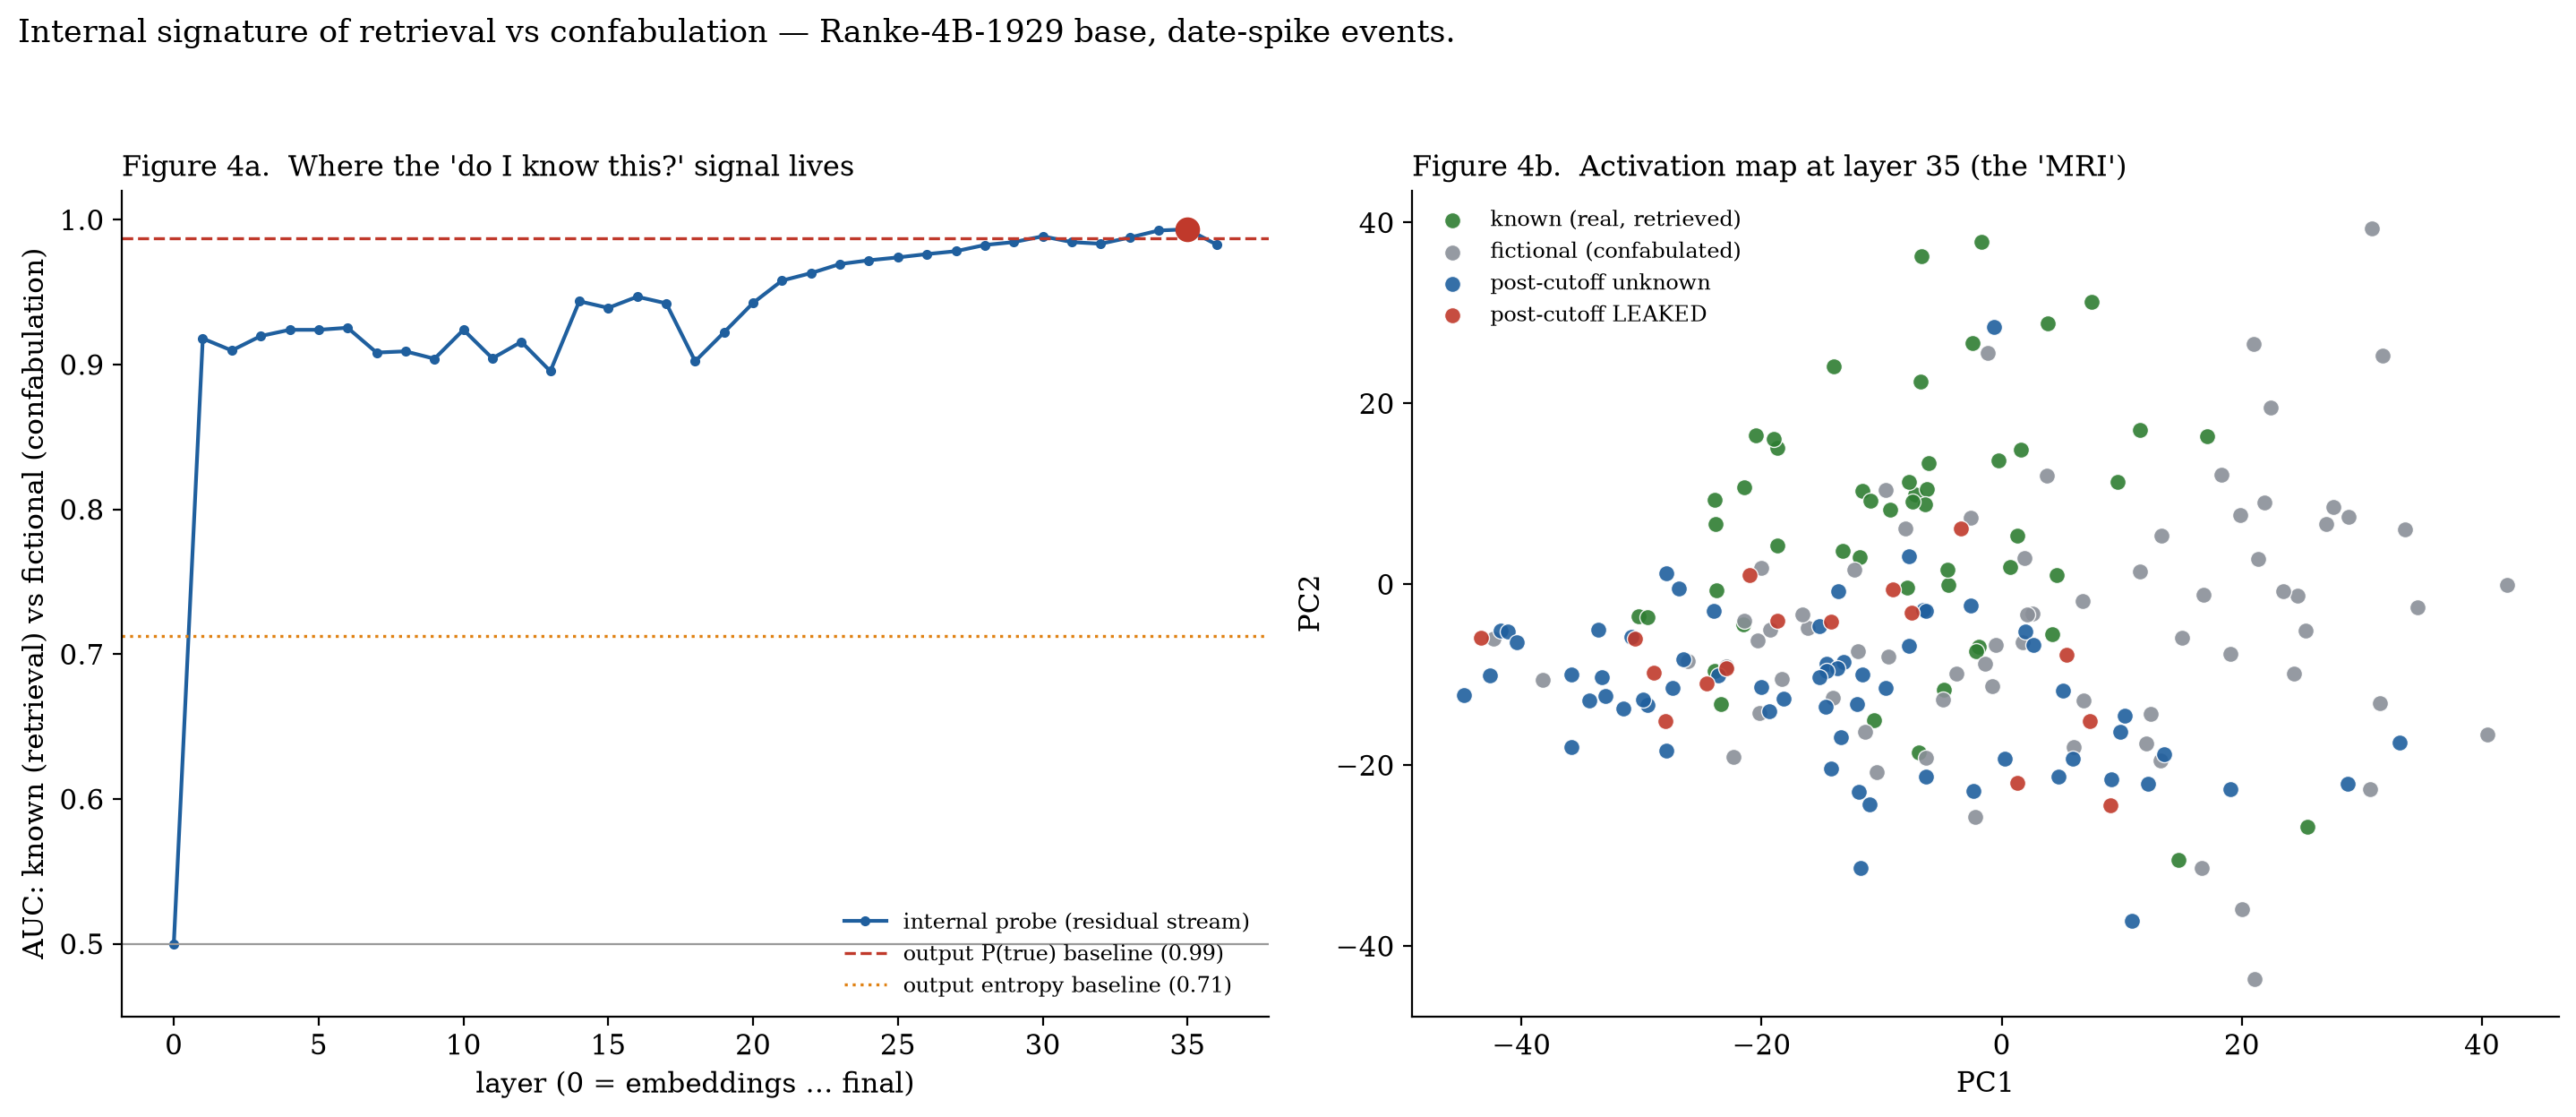
\includegraphics[width=\textwidth]{fig_probe_mri.png}
\caption{\textbf{The signature exists and generalises.} Left: 5-fold CV AUC for retrieval-vs-confabulation by layer;
the internal probe reaches $0.99$ and dominates the output-entropy baseline ($0.71$). Right: PCA of last-token states.
The probe is trained \emph{only} on known-real vs invented; post-cutoff leaked facts (red) land on the retrieval side,
genuinely-unknown post-cutoff facts (blue) on the confabulation side. Source: \code{probe\_mri.py}.}
\label{fig:pilot}
\end{figure}

On the pilot battery (50 real pre-cutoff / 70 invented / 80 post-cutoff test) the probe separates known from invented at
\textbf{AUC $0.99$} (layer 35), versus $0.71$ for a max-entropy output baseline (Fig.~\ref{fig:pilot}). Trained only on
known-vs-invented, it \emph{generalises} to two classes it never saw: mean $\mathrm{P}(\text{retrieval})$ is
$0.25$ for genuinely-unknown post-cutoff events (n$=$64) and $0.70$ for the post-cutoff events the model \emph{leaked}
(n$=$16). That split is the contamination signal, read from the inside.

\paragraph{Causal control (ROME injection).} Correlational probes invite the objection that they read surface
familiarity, not memory. We refute it causally: using a ROME-style rank-1 edit \cite{rome} to a single mid-layer MLP
down-projection, we \emph{write a date into a fake treaty}, holding the prompt byte-identical. The behavioural insert
always takes ($\mathrm{P}(\text{true})$: $3$--$13\%\!\to\!84$--$96\%$); the meter flips $2/5$ facts fully to
``retrieved'' at the read-out layer \emph{even though all five now state the year confidently}. Because only weights,
never surface, changed, a flip proves the probe reads the fact; and because a confident output alone does not force a
flip, the probe reads \emph{naturally-stored} memory rather than the answer (\code{rome\_inject.py},
\code{rome\_flip\_by\_layer.py}). The two real-treaty controls sharpen this: \emph{Locarno} (1925, a treaty the model
already remembers) reads $1.00\!\to\!1.00$---no flip, nothing to plant; \emph{Bj\"ork\"o} (1905, which the model lacks)
flips $0.00\!\to\!1.00$ when the true fact is planted.

\begin{figure}[t]\centering
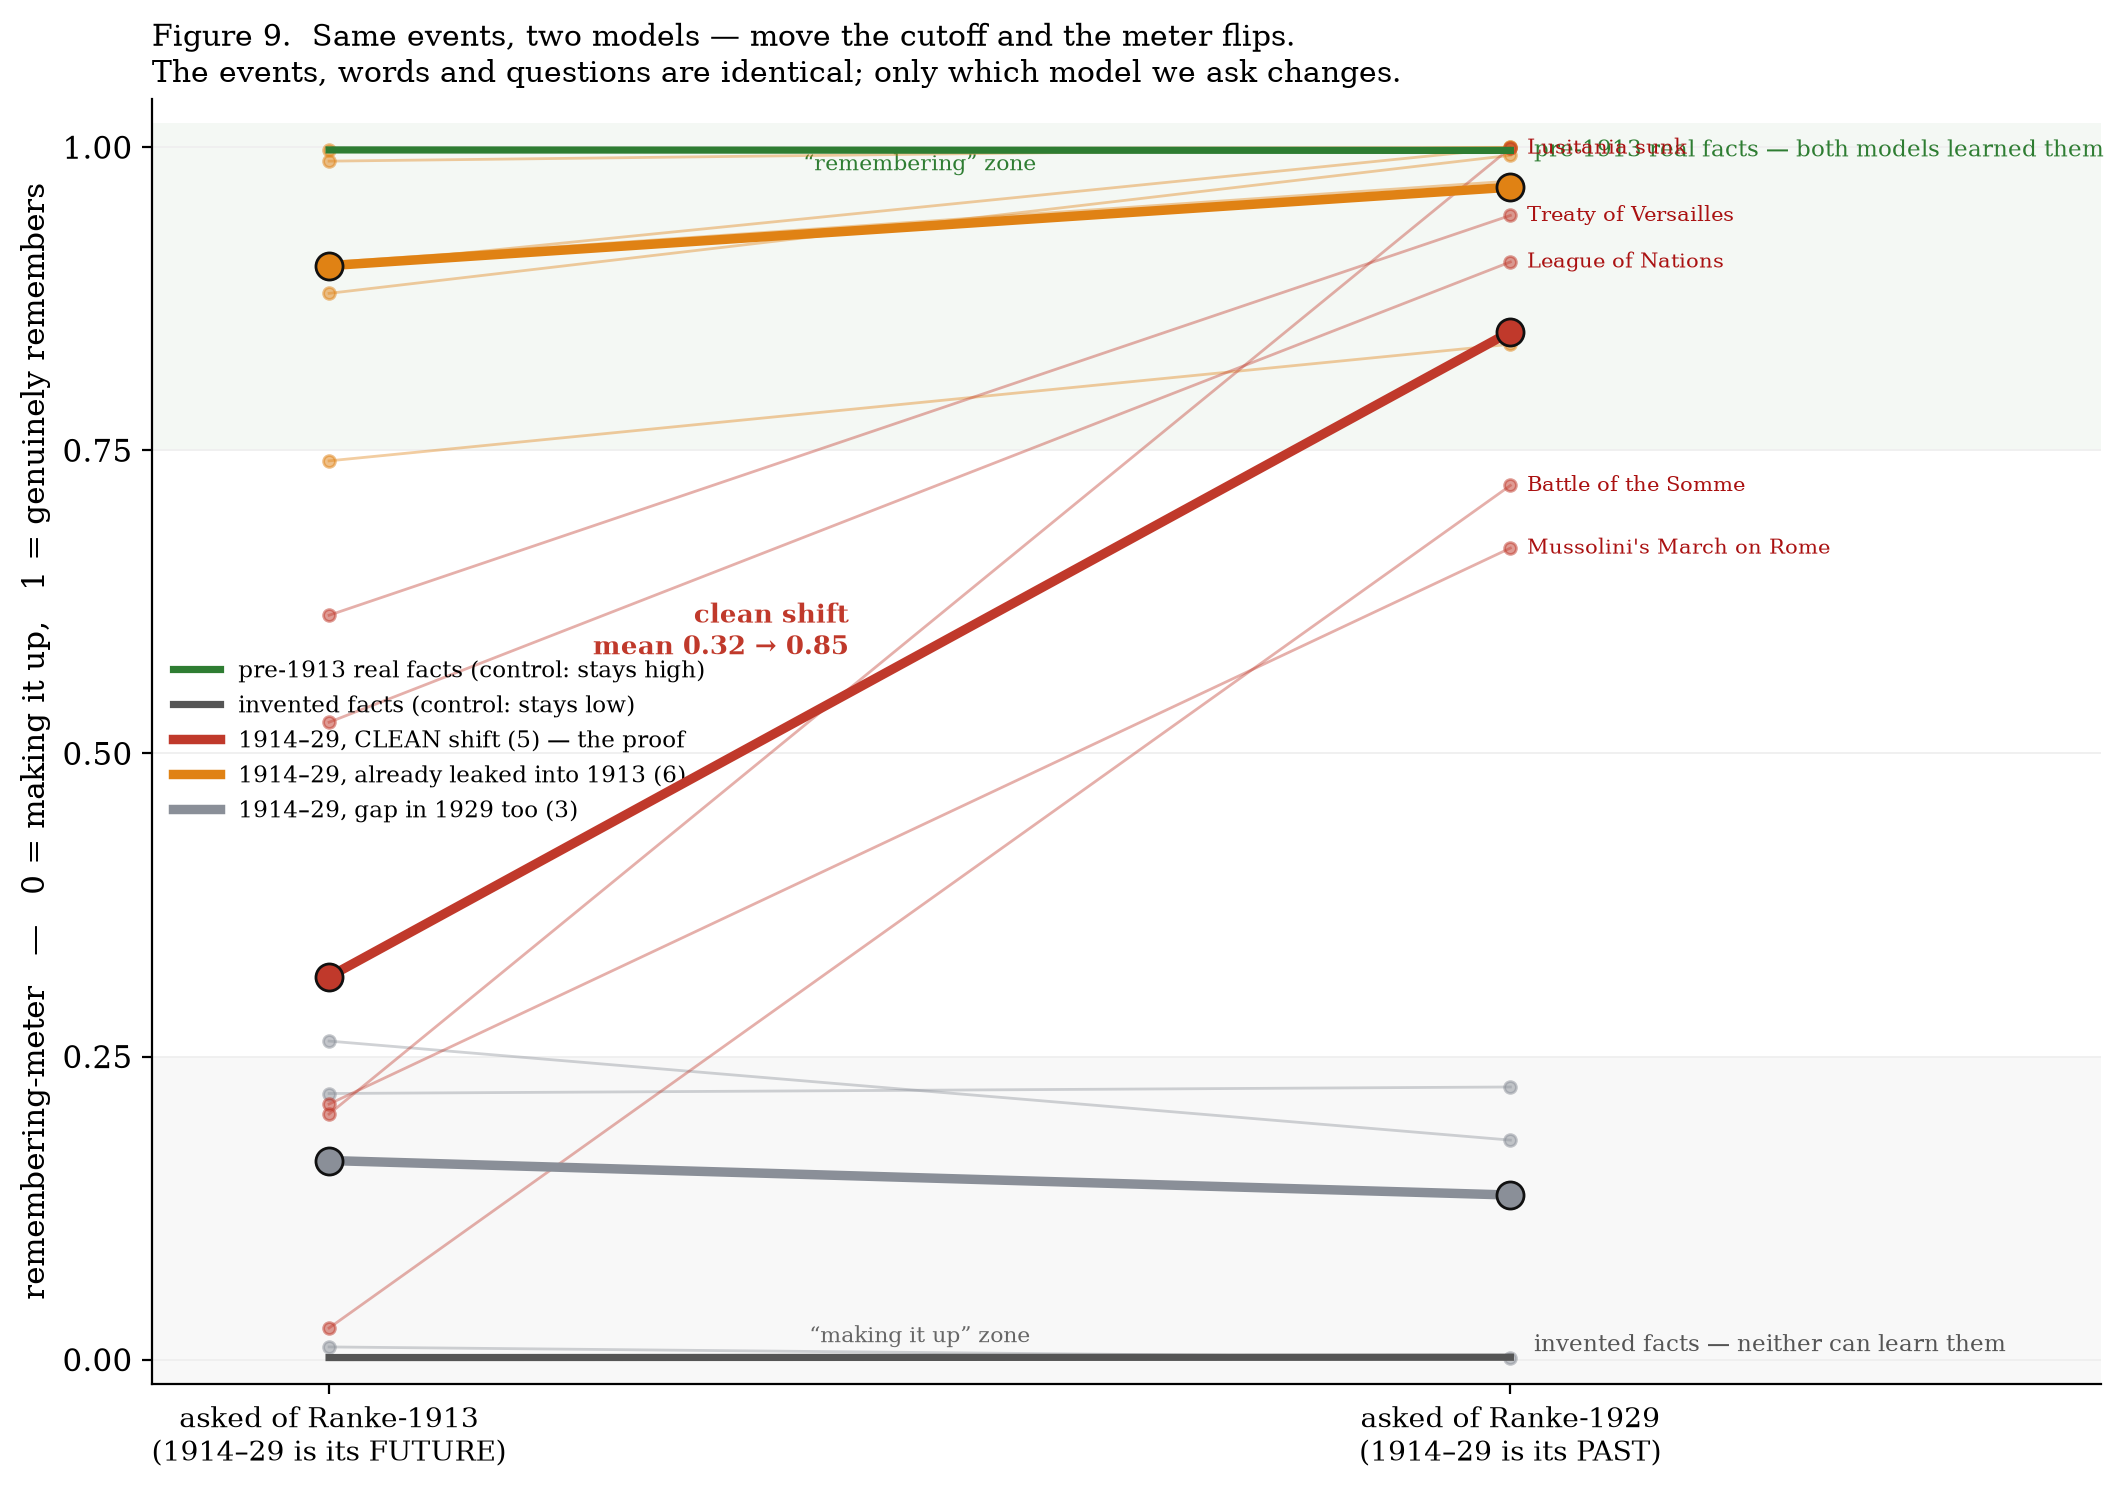
\includegraphics[width=0.92\textwidth]{fig_cutoff_shift.png}
\caption{\textbf{Two models, one cutoff apart.} The identical 1914--29 events, read by Ranke-1913 (their future) and
Ranke-1929 (their past), each with its own meter. Clean cases climb $0.32\!\to\!0.85$; pre-1913 real facts stay high on
both, invented facts stay low on both. The two ``non-shift'' groups are themselves diagnostic: events already leaked into
1913, and events Ranke-1929 never learned. Source: \code{cutoff\_shift.py}.}
\label{fig:cutoff}
\end{figure}

\paragraph{The cleanest demonstration (no editing).} Score the \emph{same} 1914--29 events on two models a cutoff apart
(Fig.~\ref{fig:cutoff}). For Ranke-1913 these are the future; for Ranke-1929, the past. The meter---each model's own---
climbs from $0.32$ to $0.85$ on the clean cases, while pre-1913 controls stay high on both and invented controls stay
low on both. Only the training window changed.

\section{Failure modes (read this before trusting a number)}\label{sec:fail}
\begin{figure}[t]\centering
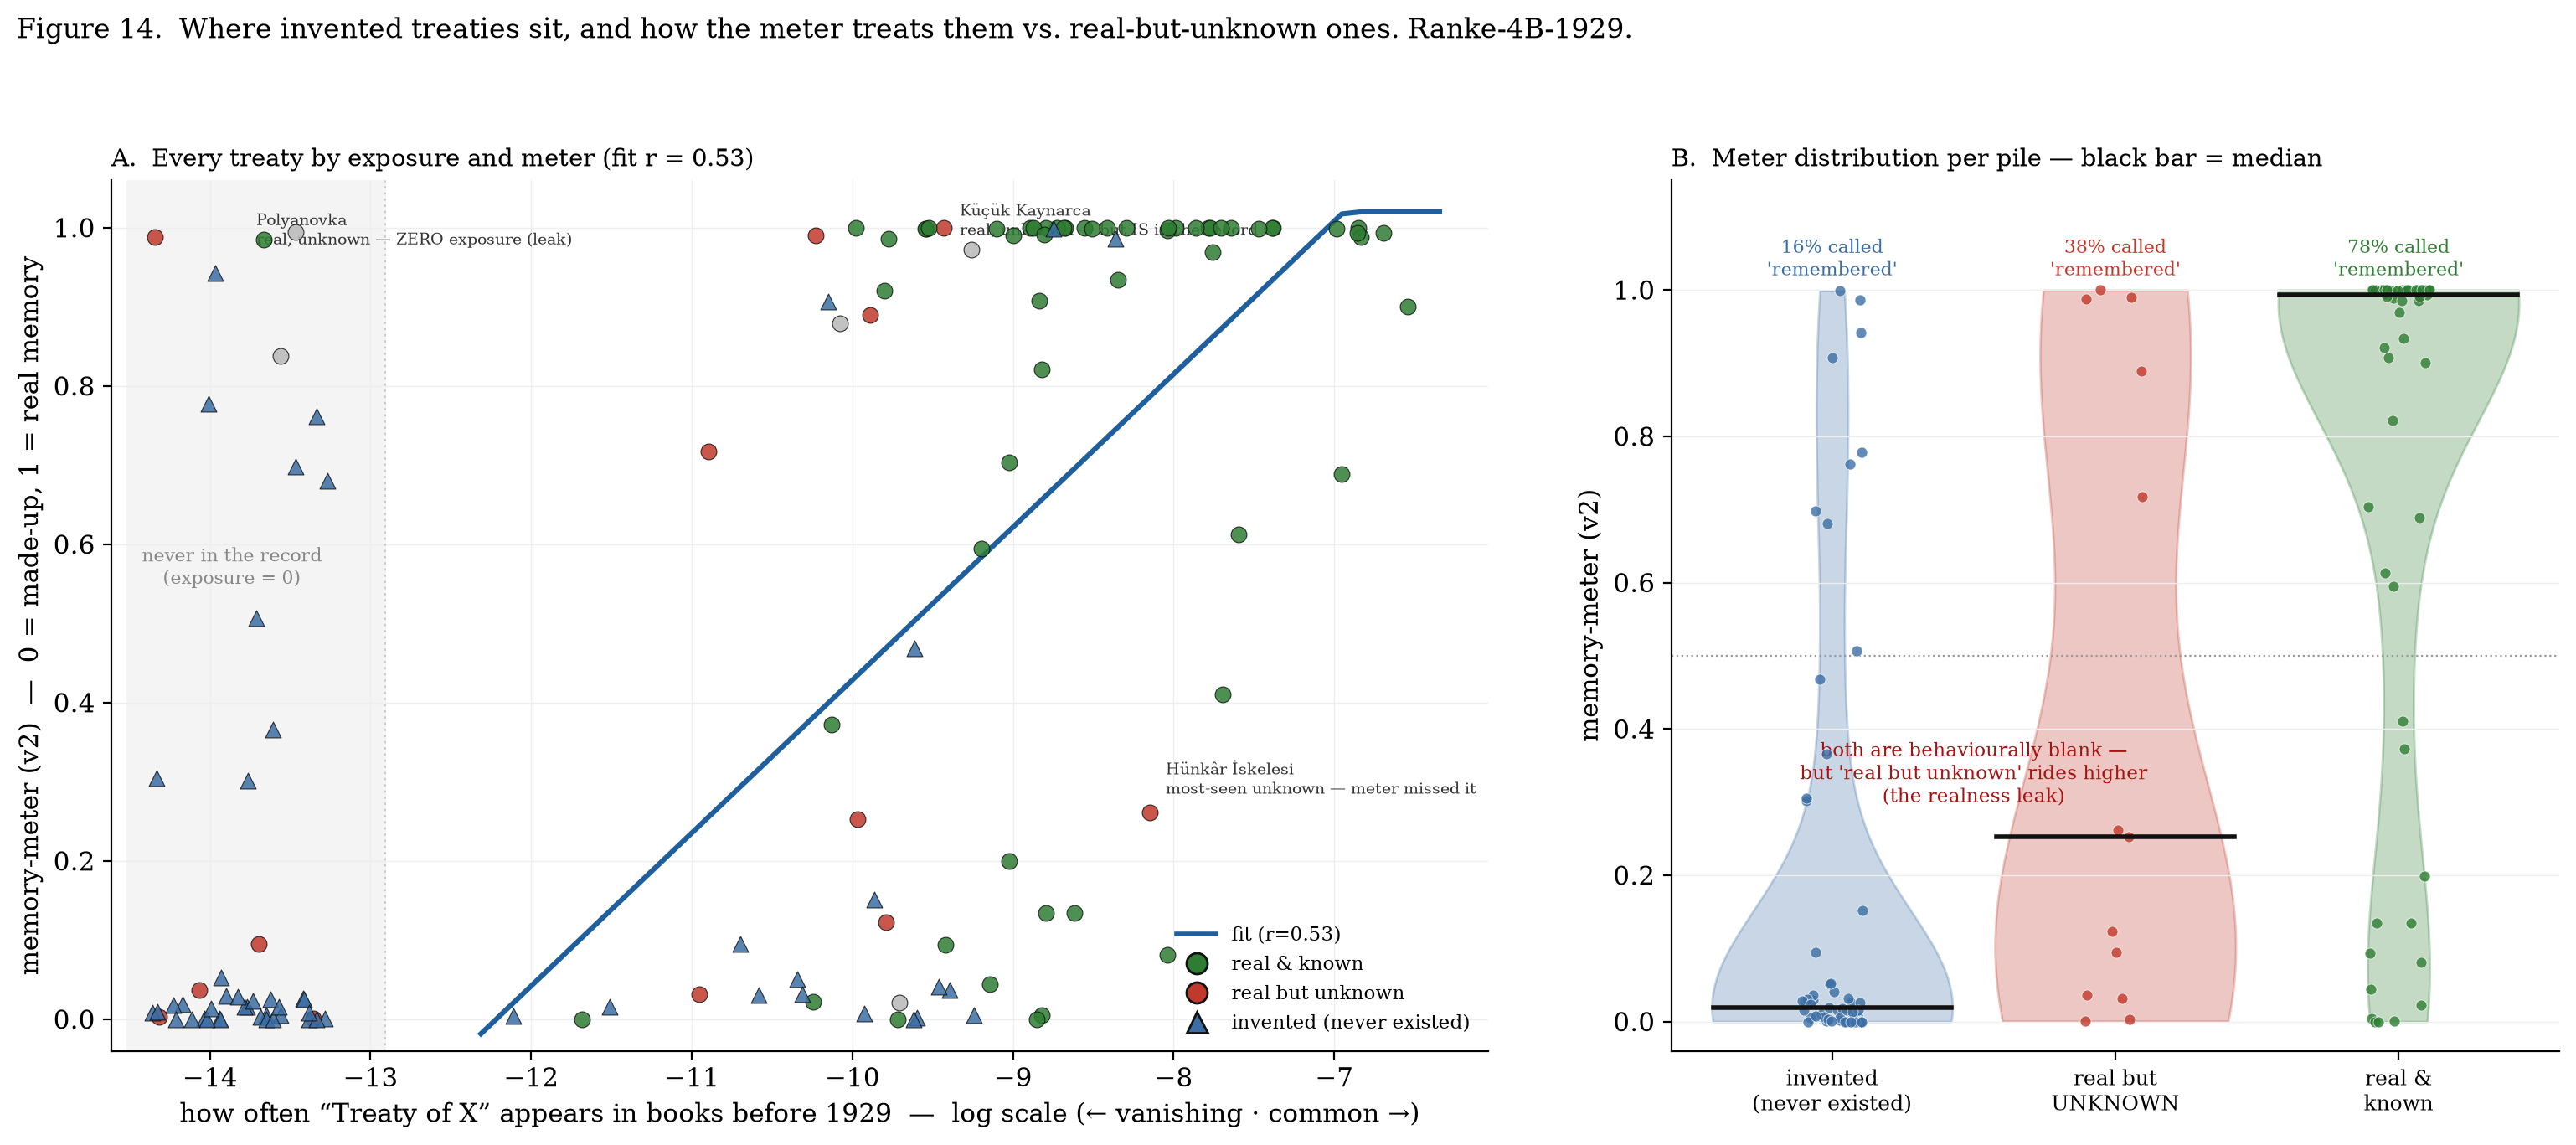
\includegraphics[width=0.86\textwidth]{fig_exposure_violins.png}
\caption{\textbf{The realness leak, made visible.} Meter distribution for invented, real-but-unknown, and real-known
treaties. Invented and real-but-unknown are \emph{both} behaviourally blank, yet real-but-unknown rides higher
($38\%$ vs $16\%$ called ``remembered''; medians $0.25$ vs $0.02$). That gap---same absence of recallable memory, only
real-vs-fake differs---is a bias toward ``this is a real thing''. Known towers over both (median $0.99$), so memory is
still the dominant signal. Source: \code{make\_exposure\_figs.py}.}
\label{fig:violin}
\end{figure}

The meter is not a black box you can trust blindly. Four documented failure modes, each with a controlled measurement:

\textbf{(1) It is not just output confidence.} Among real-name fakes, some are \emph{confident} confabulations (the model
states a firm year for a non-existent treaty: Bordeaux $80\%$, Rotterdam $77\%$). Matching real memories against these
confident lies---both output-confident by construction---the probe separates them at AUC $\mathbf{0.92}$ while the model's
own confidence manages only $0.76$ (\code{real\_entity\_null.py}). The interior betrays the lie the output hides.

\textbf{(2) It is not sentence shape or word familiarity.} A minimal-pair test---real ``Treaty of X'' vs fake
``Treaty of X'', real cities on both sides, identical template---still separates at AUC $\mathbf{0.98}$ vs $0.93$ for
output confidence (\code{minimal\_pairs.py}). Backwards example: the model rates the \emph{fake} ``Treaty of Le Havre''
$72\%$ confident and the \emph{real} ``Treaty of Portsmouth'' (1905) only $12\%$; the meter gets both right.

\textbf{(3) It carries a ``realness'' bias out of distribution (the important one).} Fig.~\ref{fig:violin}: invented and
real-but-unknown treaties are both behaviourally blank, yet the meter rates real-but-unknown ones higher. On genuinely
obscure real treaties the meter drops from $\sim\!0.98$ to $\sim\!2/3$ correct, with hard false positives
(K\"u\c{c}\"uk Kaynarca reads $0.99$ though the model knows neither its date nor its signatories) confirmed by an
independent ``who signed it?'' probe (\code{obscure\_real\_parties.py}). Interpretation: the meter partly reads
\emph{presence in the record}. We quantified this with Google Books frequency (pre-1929): meter vs
$\log$-exposure correlates $r{=}0.40$; behaviourally-known treaties have $\sim\!165\times$ the exposure of unknown ones,
so the ``unknown'' label is fair; but the meter's false positives sit at higher exposure than its correct rejections,
so \emph{some} of its ``errors'' are faint-trace catches rather than pure leak (\code{ngram\_exposure.py}). This is a
real ceiling---though \S\ref{sec:orthog} closes most of it by orthogonalisation; it is why we never report the meter alone as ground truth.

\textbf{(4) It is phrasing-sensitive.} A single arbitrary prompt under-counts, badly---see \S\ref{sec:wording}.

\paragraph{v1$\to$v2: relabelling helps but does not cure.} Training the probe to predict \emph{memory} (with
real-but-unknown moved into the negative class), rather than \emph{realness}, cuts false positives from $25$ to $14$ and
lifts AUC-vs-truth from $0.78$ to $0.86$ (Fig.~\ref{fig:cm}, \code{memory\_detector.py}); $14$ false positives remain, most of which we then close by orthogonalisation (\S\ref{sec:orthog}).

\section{Closing the realness leak by orthogonalisation, and a multi-category test}\label{sec:orthog}
The realness bias of \S\ref{sec:fail} is not a fixed cost. The leak is, by construction, the meter separating
\emph{real} from \emph{fake} \emph{among items the model does not remember}; so we remove it at the source. Within the
no-memory set we find the linear direction that best distinguishes real-but-blank from invented and project it out,
iterating until realness is no longer linearly decodable there (null-space projection, INLP-style \cite{inlp}); then we
fit the memory probe on the nulled residual. The probe can no longer lean on realness---only genuine recall separates
known from blank. Everything below is cross-validated (null directions and probe fit on the train fold, applied
out-of-fold) and GPU-free from the saved activations (\code{memory\_detector\_v3.py}).

\paragraph{On the treaty battery.} At a safe operating point ($\sim\!13$ nulled directions) the leak collapses while
memory is preserved: the correlation between the meter and pre-1929 book-exposure among behaviourally-unknown treaties
falls $+0.33\!\to\!-0.13$; the real-unknown-vs-invented gap $+0.21\!\to\!+0.05$; the leak AUC $0.69\!\to\!0.57$; and
memory AUC (real-known vs real-unknown) \emph{rises}, $0.86\!\to\!0.90$. The note's worst false positive,
K\"u\c{c}\"uk Kaynarca, drops $0.35\!\to\!0.19$ (correctly ``not remembered''); on held-out obscure treaties the studied
stay high ($0.92\!\to\!0.91$) and the unstudied fall ($0.24\!\to\!0.16$). A \textbf{cliff} bounds it: nulling past
$\sim\!18$ directions destabilises the out-of-distribution treaties (K\"u\c{c}\"uk Kaynarca rebounds to $0.77$); the win
is robust across $10$--$18$ directions, so we stop there (\code{memory\_detector\_v3\_sweep.py}).

\paragraph{A 278-item, five-category, adversarial battery.} To test generalisation we built a battery across wars,
Nobel laureates, painters, novelists and US presidents, in four classes: real-famous, real-obscure, invented, and
\emph{false-fact} (real famous non-presidents framed as president---a real name attached to a memory that cannot exist).
The $216$ real entities were verified against Wikipedia; the $62$ invented ones were verified \emph{non-existent};
memory is labelled behaviourally (studied vs blank) as before. Of $278$ items, $39$ are studied and $167$ blank
($117$ real-but-blank, $50$ invented) (\code{bignull\_battery.py}, \code{bignull\_extract.py}, \code{bignull\_analyze.py}).
Three findings (Fig.~\ref{fig:bignull}):
\begin{enumerate}\itemsep1pt
\item \textbf{Memory generalises}: the meter separates studied from blank at \textbf{AUC $0.95$} across all five
categories---far beyond treaties.
\item \textbf{The leak is small and category-specific}: the pooled leak AUC is only $0.55$ (vs $0.69$ on treaties). It
concentrates in the \emph{person-name} categories---painters $0.68$, novelists $0.79$---where a real name carries
familiarity; wars ($0.45$) and Nobel ($0.49$) show none.
\item \textbf{The fix must be per-entity-type}: a single \emph{global} null is too blunt---it over-corrects wars
($0.45\!\to\!0.32$) and \emph{worsens} painters ($0.68\!\to\!0.76$), because ``a real painter-name'' and ``a real
war-name'' are different directions. Nulling realness \emph{within each category} closes them: painters
$0.68\!\to\!0.52$, novelists $0.79\!\to\!0.54$, overall $0.55\!\to\!0.48$, memory kept ($0.94$).
\end{enumerate}

\begin{figure}[t]\centering
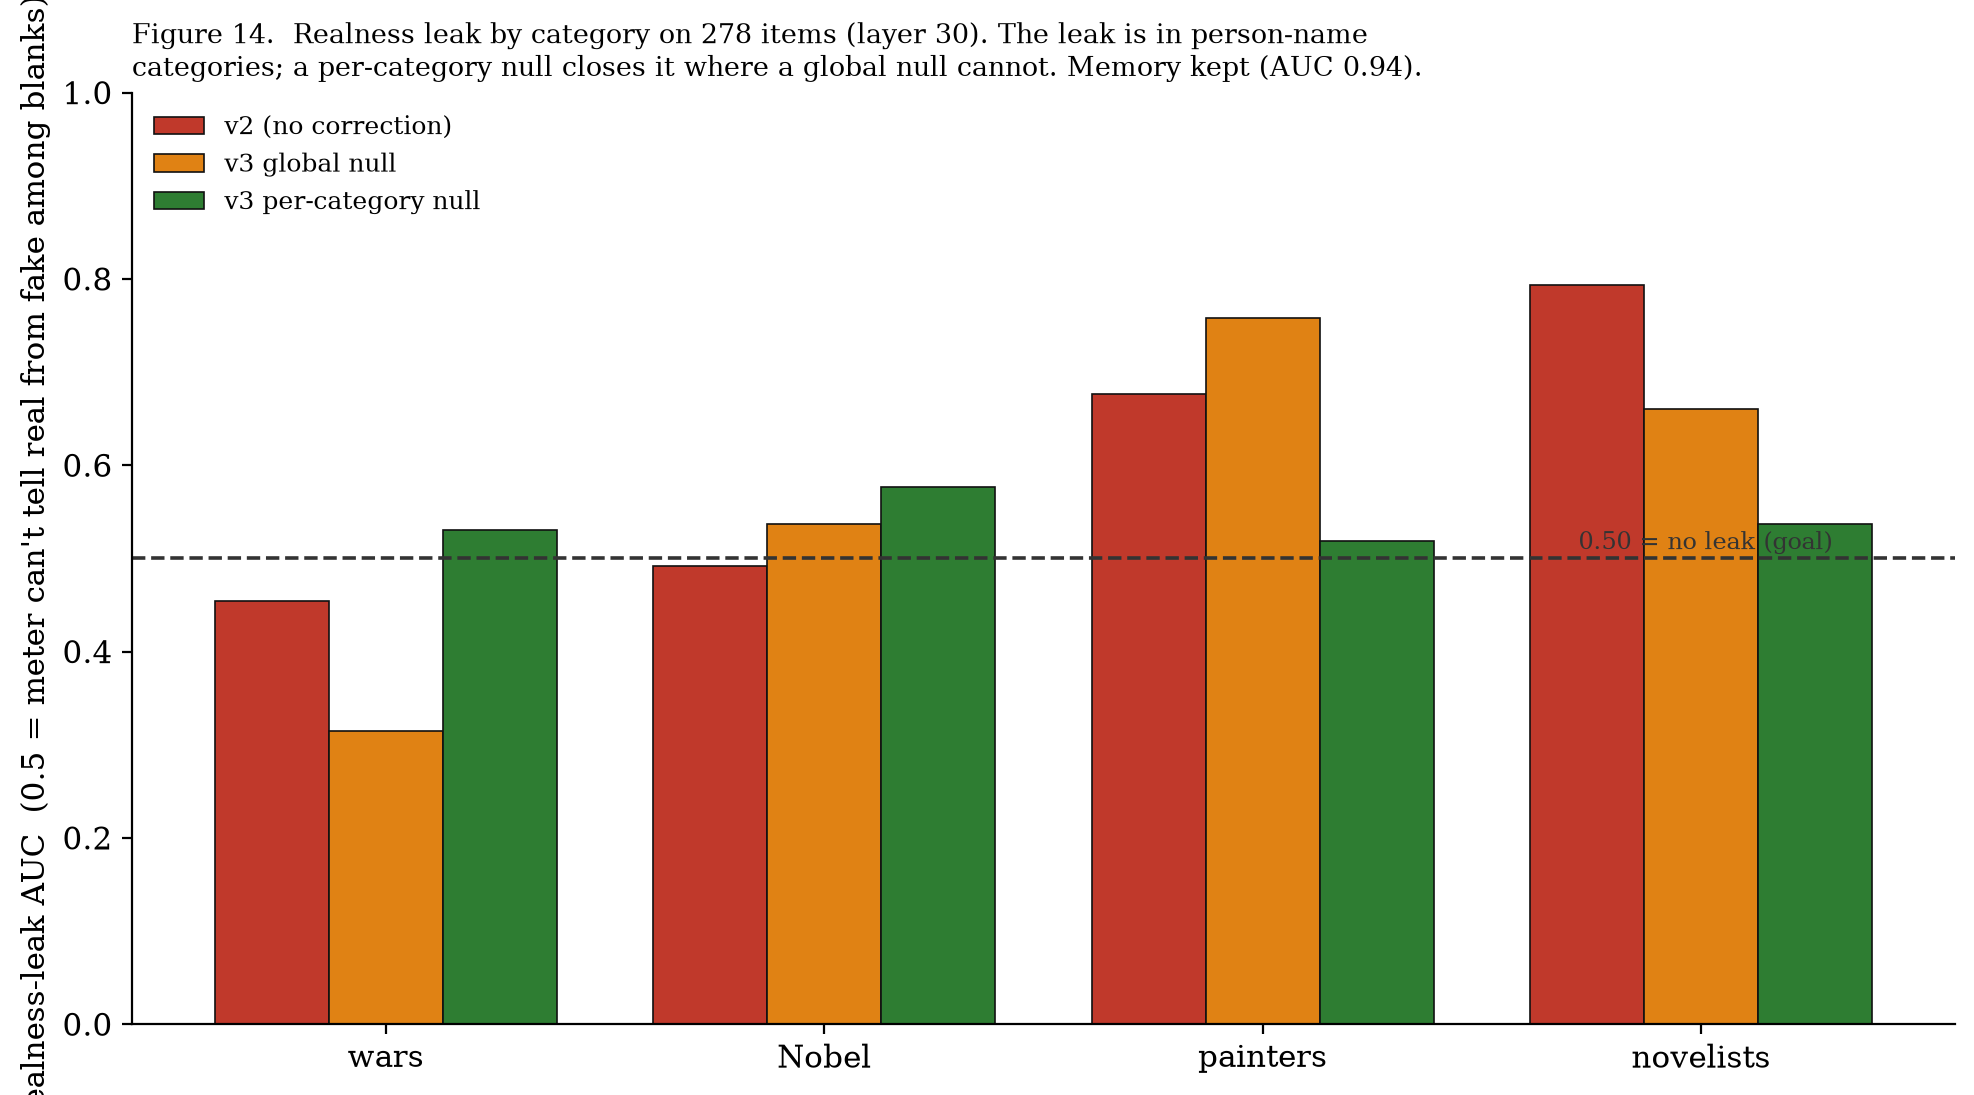
\includegraphics[width=0.9\textwidth]{fig_bignull_v3.png}
\caption{\textbf{The realness leak is category-specific, and closes per entity-type.} Realness-leak AUC (real-blank vs
invented among no-memory items; $0.5$ = no leak) by category, for three meters: no correction, a global null, and a
per-category null. The leak lives in the person-name categories; the global null over/under-corrects; the per-category
null brings every category to $\approx\!0.5$ while memory AUC stays $0.94$. Source: \code{bignull\_analyze.py}.}
\label{fig:bignull}
\end{figure}

\paragraph{Honest residuals, and the meter's proper role.} The president category has no invented items to contrast, so
it cannot be realness-nulled directly; person-name directions bleed into it and nudge the false-fact class
$0.22\!\to\!0.46$ ($\approx$chance---not fooled into ``remembered'', but a residue); adding fake-name presidents would
settle it. The operational lesson is a \emph{division of labour}. For \emph{whether the model knows a date} the
behavioural year-spike is the clean primary signal---it carries no realness bias by construction. The meter's
distinctive, now-validated contribution is the narrower case the year-spike cannot handle: telling a genuine memory from
a \emph{confident confabulation}, where a firm fake or wrong answer fools the output but not the interior
(\S\ref{sec:fail}, the $0.92$-vs-$0.76$ result; the false-fact ``President Franklin'' correctly read as not-remembered).
Neither is proof: both are pre-filters that feed the corpus check (\S\ref{sec:rome}). And realness is
category-specific---a real name means different things for a war and a painter---so any realness correction belongs
inside each entity type.

\begin{figure}[t]\centering
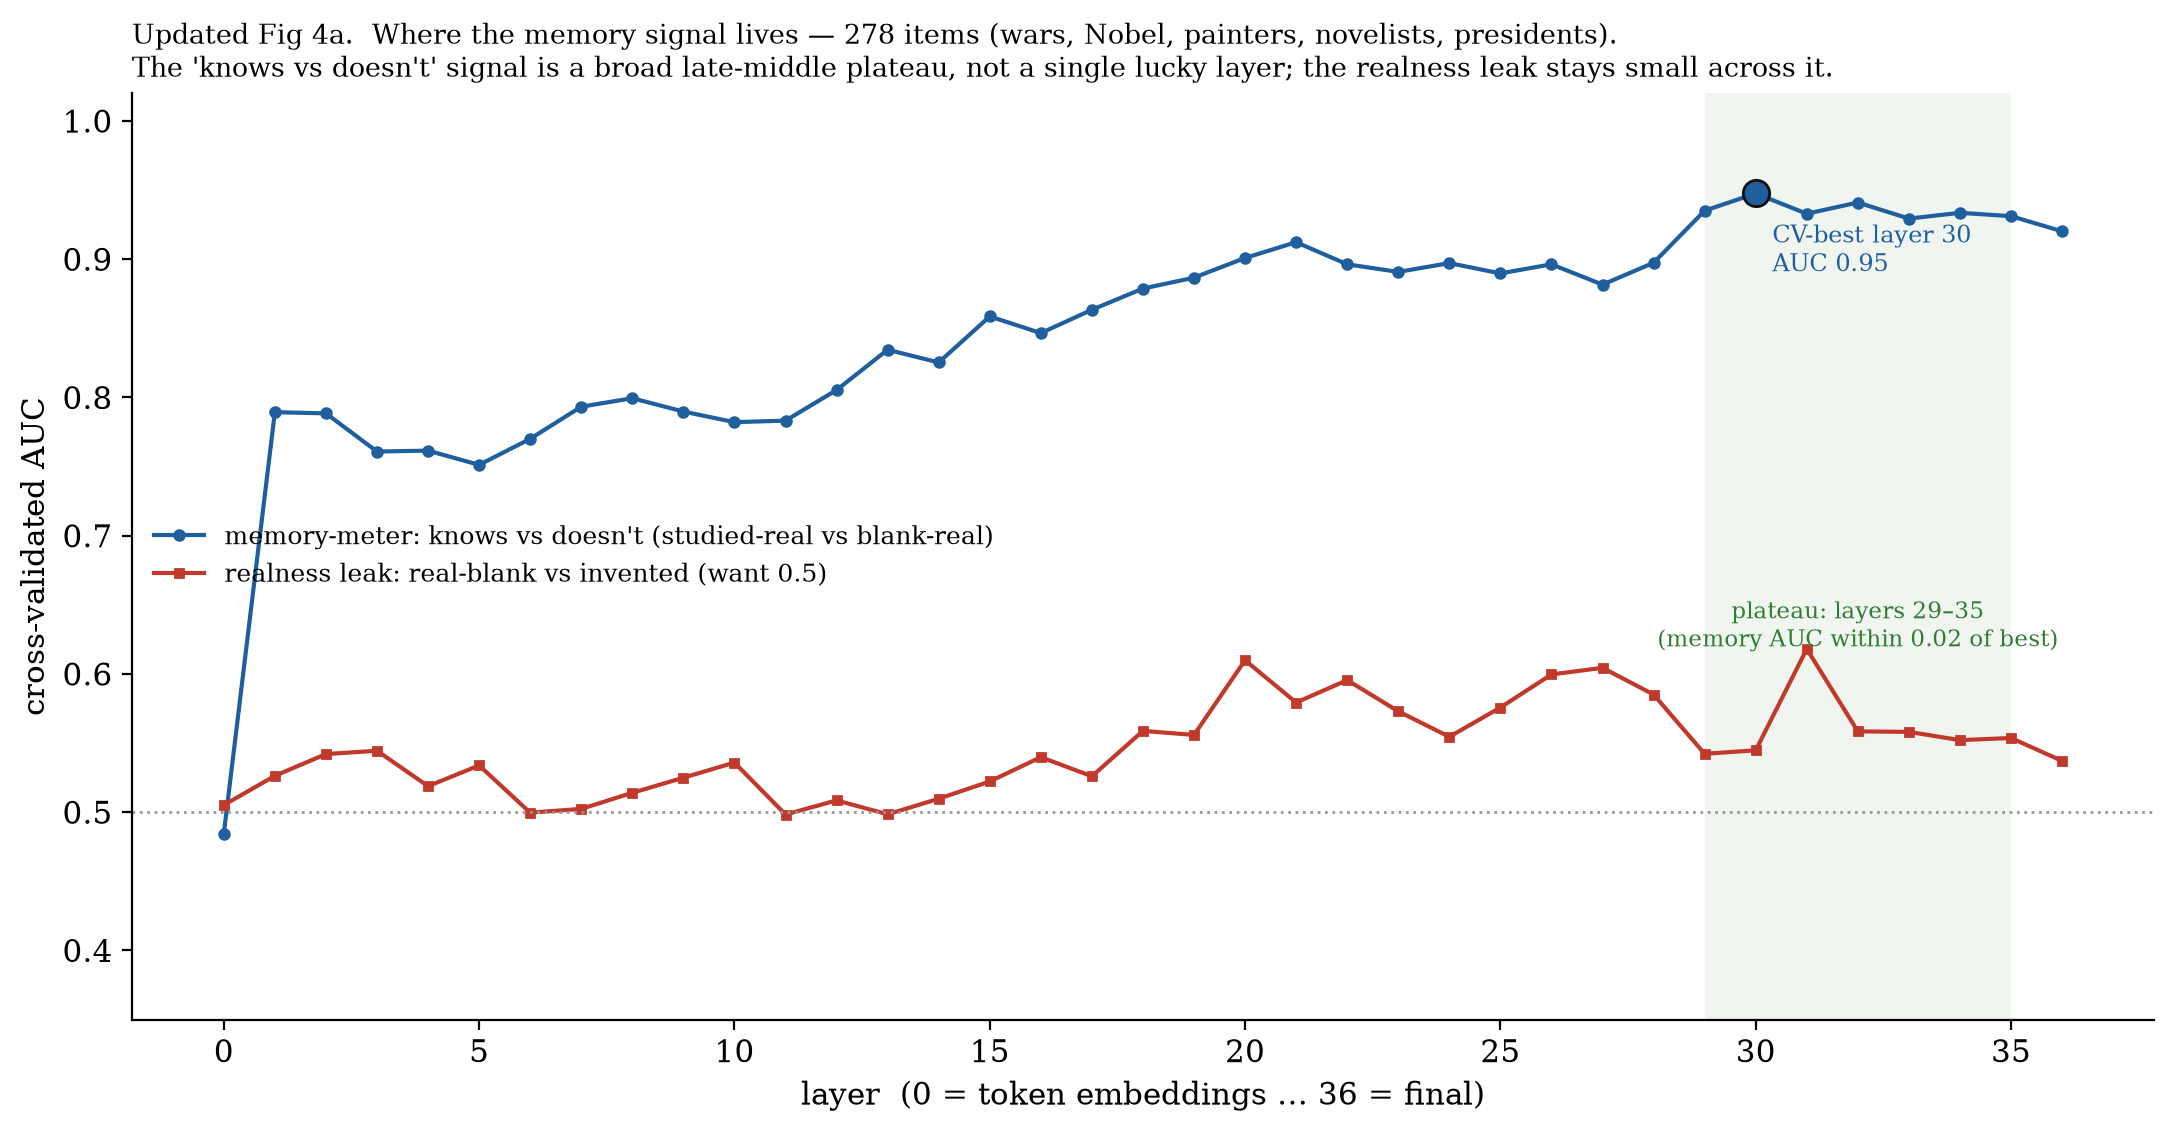
\includegraphics[width=\textwidth]{fig_layer_curve_big.png}
\caption{\textbf{The memory signal is a broad plateau, not a lucky layer} (updates the pilot layer panel,
Fig.~\ref{fig:pilot}, on the 278-item, memory-labelled battery). The meter's cross-validated AUC (knows vs doesn't;
studied-real vs blank-real) sits within $0.02$ of its best across layers $29$--$35$ (CV-best $30$, AUC $0.95$); the
realness leak (red; want $0.5$) stays modest across the same band. Source: \code{layer\_curve\_big.py}.}
\label{fig:layercurve}
\end{figure}

\section{Operational leak detection: combine the two signals}\label{sec:combine}
\begin{figure}[t]\centering
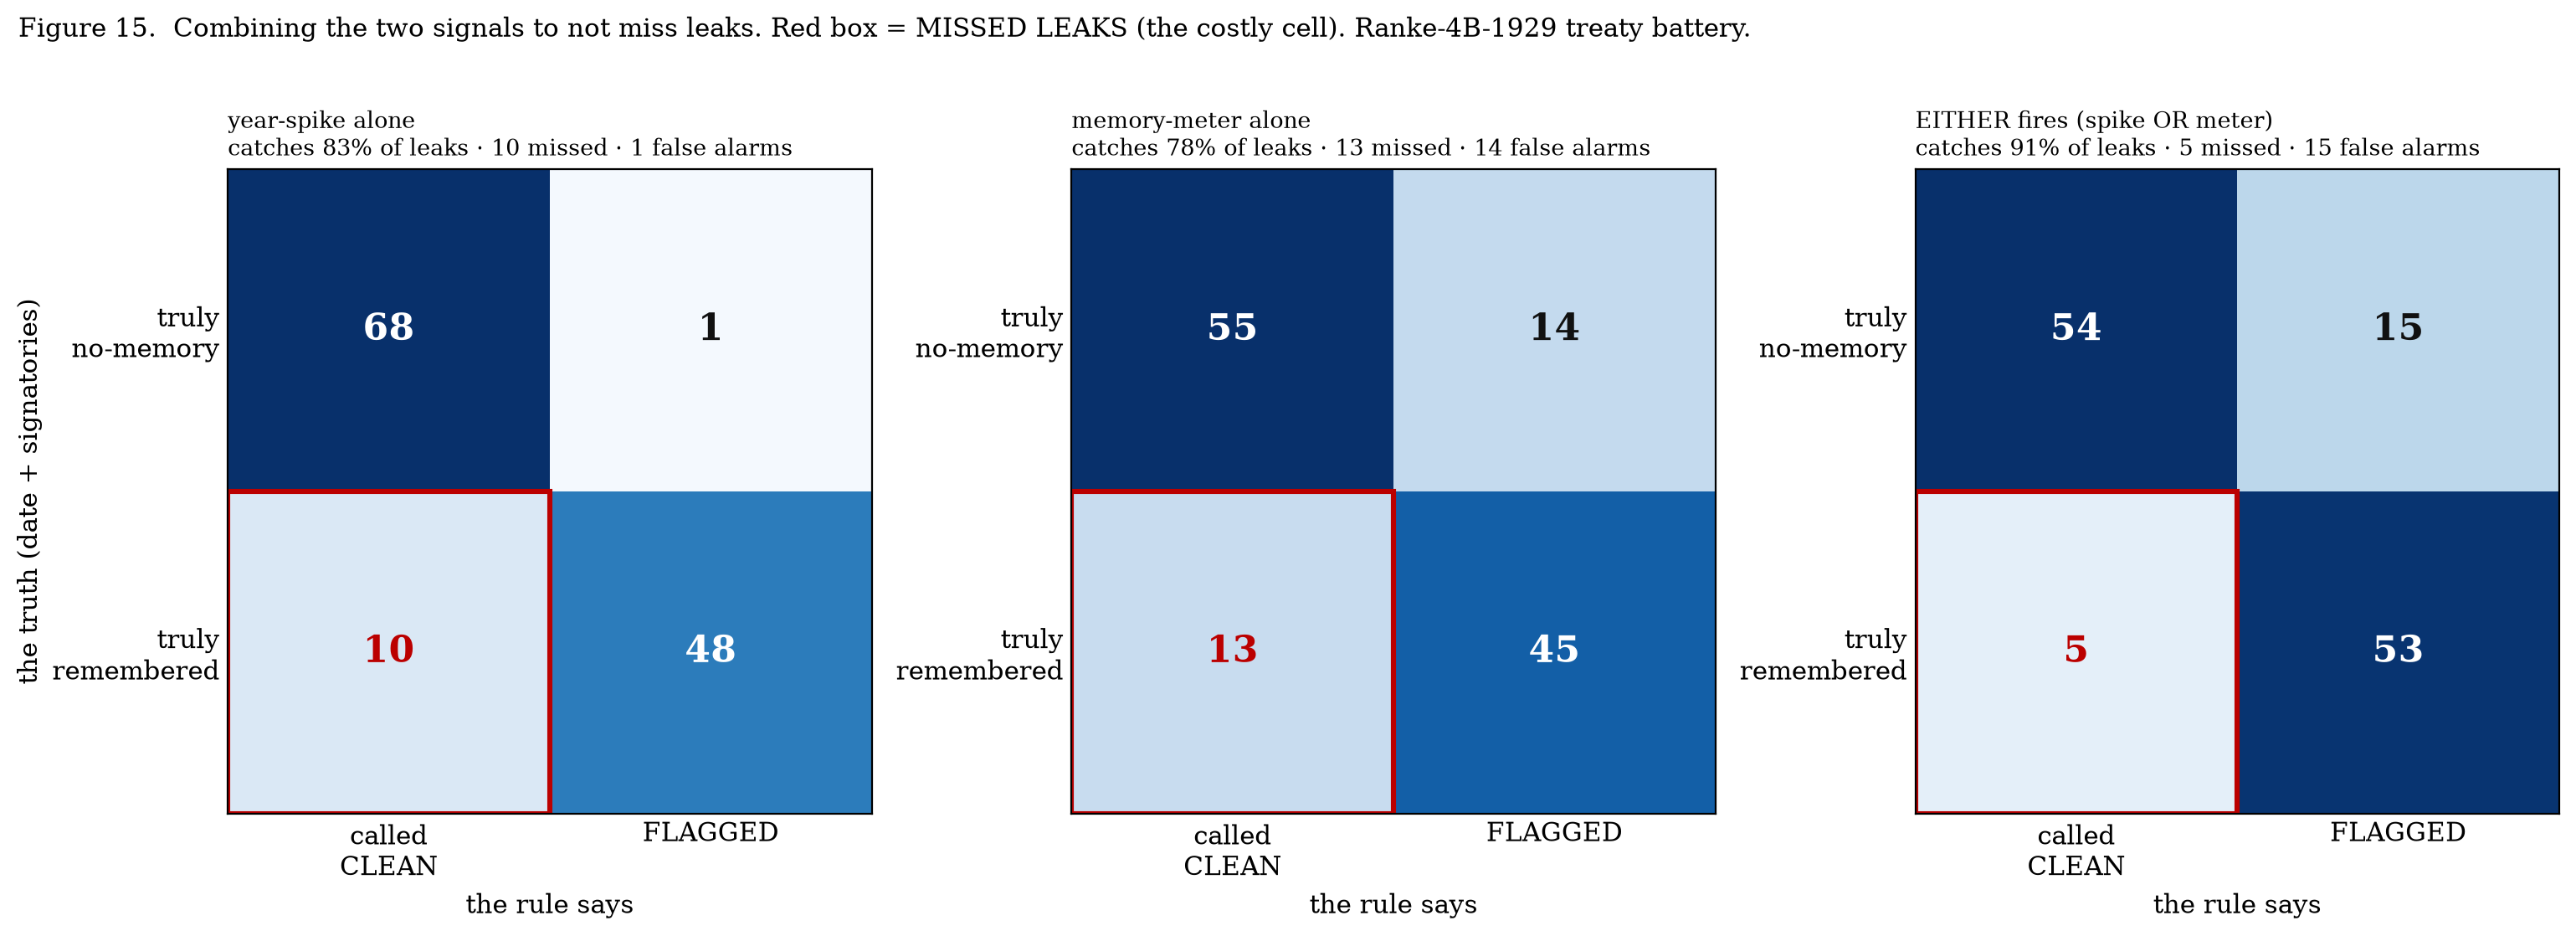
\includegraphics[width=\textwidth]{fig_combined_rule.png}
\caption{\textbf{Two-signal leak rule.} Flag a fact if the year-spike \emph{or} the meter fires. Red box = missed leaks
(the costly cell). OR-ing halves missed leaks ($10\!\to\!5$; recall $83\%\!\to\!91\%$) because the detectors miss
different things---the spike misses facts known through non-date attributes, the meter catches five of them---at the cost
of the meter's realness false alarms ($1\!\to\!15$). For leak-hunting that is the right trade. Source:
\code{combined\_rule.py}.}
\label{fig:cm}
\end{figure}

For a contamination audit the asymmetry is stark: a \emph{missed leak} lets contamination through silently, whereas a
\emph{false alarm} merely triggers a manual re-check. So we OR the signals---flag a fact unless it shows neither a
year-spike nor a high meter. On the treaty battery (58 truly-remembered, 69 not), against the two-signal ground truth
(known $=$ nails date \emph{or} signatories):
\begin{center}\small
\begin{tabular}{lcccc}\toprule
rule & recall & missed leaks & false alarms & precision\\\midrule
year-spike alone & $0.83$ & $10$ & $1$ & $0.98$\\
memory-meter alone & $0.78$ & $13$ & $14$ & $0.76$\\
\textbf{either fires (OR)} & $\mathbf{0.91}$ & $\mathbf{5}$ & $15$ & $0.78$\\\bottomrule
\end{tabular}
\end{center}
The two detectors are complementary: the meter recovers leaks the date-spike cannot see (facts recalled without a
retrievable date). Caveat: the year-spike is part of the ground-truth definition here, so its precision column is
optimistic; the meter's genuine contribution is the five extra leaks it catches.

\section{Fixing phrasing sensitivity: the ``best-wording'' normalisation}\label{sec:wording}
Both indicators depend on how the fact is phrased, because a phrase the model saw often in text is one it recognises and
dates best. A single arbitrary prompt therefore \emph{under-counts}. The principled fix: for each event, score several
specific phrasings and (i) pick the \emph{most natural} one---the wording the model itself finds most fluent, i.e.
maximal mean per-token log-probability of the prefix (a cheap proxy for ``most likely in a book'')---or (ii) take the
max indicator over the set (the most sensitive detector, with a mild multiple-comparison caveat).
\begin{lstlisting}
def fluency(prompt):                       # higher = more natural to the model
    ids = tok(prompt, add_special_tokens=False).input_ids
    with torch.no_grad():
        lp = torch.log_softmax(model(torch.tensor([ids],device=model.device)).logits[0].float(), -1)
    return float(np.mean([lp[k-1, ids[k]].item() for k in range(1, len(ids))]))
best = max(phrasings, key=fluency)         # then score year-spike + meter under `best`
\end{lstlisting}
The effect is large and vindicates the concern (\code{best\_wording.py}):
\begin{center}\small
\begin{tabular}{lccccc}\toprule
event & single meter & fluency-best meter & \textbf{max meter} & single spike & \textbf{max spike}\\\midrule
WW2 begins       & $0.36$ & $1.00$ & $1.00$ & $6\%$ & $18\%$\\
Hitler to power  & $0.27$ & $0.88$ & $0.97$ & $1\%$ & $8\%$\\
Kristallnacht    & $0.00$ & $0.00$ & $0.94$ & $5\%$ & $5\%$\\
Civil Rights Act & $0.99$ & $0.99$ & $0.99$ & $9\%$ & $\mathbf{30\%}$\\
UN founded       & $0.56$ & $0.91$ & $0.91$ & $26\%$ & $36\%$\\
\midrule
Moon landing (ctl) & $0.04$ & $0.01$ & $0.04$ & $3\%$ & $4\%$\\
Invented (ctl)     & $0.00$ & $0.00$ & $0.00$ & $4\%$ & $4\%$\\\bottomrule
\end{tabular}
\end{center}
Recognition of the WW2/persecution/civil-rights band is recovered under a fair wording, and the Civil Rights Act's date
leaks at $30\%$ once phrased canonically---while controls stay dark even at the max. \textbf{Operational recommendation:}
for any sweep, use $\ge 5$ natural phrasings per event and report the \emph{max} of each indicator; use fluency-ranking
for a single principled point estimate. The wide-net sweep (\code{wide\_net.py}) used one prompt per event and therefore
\emph{understates} contamination; it should be re-run in max-over-phrasing mode.

\paragraph{Ideas for the phrasing set (formulations).} (a) verb/voice variants (``was signed'' / ``was concluded'' /
``signing took place''); (b) entity-forward vs event-forward (``Germany invaded Poland'' vs ``the Second World War
began''); (c) canonical named forms mined from the model itself (greedy-decode ``The event known as \_\_ happened in'');
(d) register variants (encyclopedic vs narrative); (e) multilingual restatements (contamination often enters via
non-English text); (f) cloze at the entity rather than the date (``The 1945 surrender of \_\_'') to separate
date-recall from entity-recall; (g) distractor-controlled minimal pairs (swap the true entity for a plausible fake to
net out template effects). Aggregate by max (sensitivity) and by fluency-weighted mean (robust point estimate).

\section{Can editing firm up a contamination claim? A hard look, and a negative pilot}\label{sec:rome}
It is tempting to think ROME-style editing could \emph{prove} a fact is stored: if the memory is already there, inserting
it should be redundant, and inserting its \emph{negation} should meet resistance. We think this through and test it, and
the honest answer is \textbf{no---editing does not firm up contamination}, for a structural reason.

\textbf{Why the intuition fails.} ROME is engineered to be an \emph{effective} rank-1 write: it drives the target token's
probability to $\sim\!1$ regardless of the prior. Insertion success is therefore \emph{uninformative} about whether a
prior existed. The only edit-derived quantity that tracks the prior is the pre-edit loss $-\log \mathrm{P}(\text{true})$,
which is just the year-spike in log space---nothing new.

\textbf{The pilot (counterfactual resistance).} We planted a \emph{false} year on one phrasing and asked whether the
\emph{true} year survives on a paraphrase---resistance would signal an entrenched memory. It does not
(\code{rome\_contamination.py}):
\begin{center}\small
\begin{tabular}{lcc}\toprule
 & lie generalises to paraphrase & true year survives\\\midrule
KNOWN treaties (memory present) & $69\%$ & $0\%$\\
UNKNOWN treaties (no memory)    & $73\%$ & $0\%$\\\bottomrule
\end{tabular}
\end{center}
Utrecht's date went $94\%\!\to\!0\%$: the edit overwrote a strongly-held memory completely, and known and unknown
treaties are indistinguishable. A pre-existing memory does \emph{not} resist a rank-1 lie, so this route is dead.

\textbf{What does firm up contamination.} Three tools, in increasing definitiveness. (i) \emph{Membership inference}:
the model is systematically \emph{less surprised} by text it was trained on---Min-$K\%$ Prob \cite{minkprob}, calibrated
perplexity, and loss-ratio tests \cite{carlini21,carlini23}. Our best-worded year-spike is a crude special case; a
proper implementation scores the fact's \emph{canonical sentence} (not just the year) under Min-$K\%$. (ii)
\emph{Causal tracing} \cite{rome} (the diagnostic, not the editing, half of ROME): corrupt the subject embedding and
restore each layer in turn---a genuinely stored fact exhibits a causal-mediation hotspot at the subject token in
mid-layer MLPs; a confabulation does not. This we recommend and did \emph{not} yet run. (iii) The \emph{corpus check}:
grep the training data (or a period-matched proxy) for the fact---the gold standard, and the natural next step here.
The meter is best understood as a fast, learned pre-filter that flags candidates for (i)--(iii), not as proof.

\section{Replication checklist}\label{sec:repro}
\begin{enumerate}\itemsep2pt
\item Environment: \code{uv venv .venv --python 3.12}; \code{torch}, \code{transformers}, \code{scikit-learn},
  \code{numpy}, \code{matplotlib}. GPU optional (RTX 3060 sufficient; bf16). \emph{Never} put the venv in a synced folder.
\item Battery: data modules \code{events\_dates\_big.py}, \code{treaties\_battery.py}, \code{post1930\_battery.py}.
  Positives $=$ real pre-cutoff facts; negatives $=$ invented, surface-matched. For treaties, add the signatory forced-
  choice for a two-signal ground-truth label.
\item Extract last-token \code{hidden\_states[LSTAR]}; standardise with train $(\mu,\sigma)$; fit logistic regression;
  choose $\ell^\star$ by 5-fold CV AUC. Report \emph{out-of-fold} predictions only.
\item Always report the output-confidence baseline alongside the meter, and the per-group confusion
  (invented / real-known / real-unknown).
\item For any post-cutoff sweep: $\ge 5$ natural phrasings per event, report the max indicator; treat the meter as a
  candidate generator, then confirm with membership inference and a corpus check.
\item Do \emph{not} claim ``contaminated'' from the meter alone; do not read the meter on out-of-distribution surface
  (exotic names) without the exposure caveat.
\end{enumerate}

\begin{thebibliography}{99}\small
\bibitem{rome} K. Meng, D. Bau, A. Andonian, Y. Belinkov. \emph{Locating and Editing Factual Associations in GPT}. NeurIPS 2022. arXiv:2202.05262.
\bibitem{memit} K. Meng, A. Sharma, A. Andonian, Y. Belinkov, D. Bau. \emph{Mass-Editing Memory in a Transformer}. ICLR 2023. arXiv:2210.07229.
\bibitem{kadavath} S. Kadavath et al. \emph{Language Models (Mostly) Know What They Know}. arXiv:2207.05221, 2022.
\bibitem{azaria} A. Azaria, T. Mitchell. \emph{The Internal State of an LLM Knows When It's Lying}. EMNLP Findings 2023. arXiv:2304.13734.
\bibitem{burns} C. Burns, H. Ye, D. Klein, J. Steinhardt. \emph{Discovering Latent Knowledge in Language Models Without Supervision}. ICLR 2023. arXiv:2212.03827.
\bibitem{zou} A. Zou et al. \emph{Representation Engineering: A Top-Down Approach to AI Transparency}. arXiv:2310.01405, 2023.
\bibitem{alain} G. Alain, Y. Bengio. \emph{Understanding intermediate layers using linear classifier probes}. arXiv:1610.01644, 2016.
\bibitem{logitlens} nostalgebraist. \emph{interpreting GPT: the logit lens}. LessWrong, 2020.
\bibitem{tunedlens} N. Belrose et al. \emph{Eliciting Latent Predictions from Transformers with the Tuned Lens}. arXiv:2303.08112, 2023.
\bibitem{minkprob} W. Shi et al. \emph{Detecting Pretraining Data from Large Language Models} (Min-$K\%$ Prob). ICLR 2024. arXiv:2310.16789.
\bibitem{inlp} S. Ravfogel, Y. Elazar, H. Twiton, Y. Goldberg. \emph{Null It Out: Guarding Protected Attributes by Iterative Nullspace Projection}. ACL 2020. arXiv:2004.07667.
\bibitem{carlini21} N. Carlini et al. \emph{Extracting Training Data from Large Language Models}. USENIX Security 2021. arXiv:2012.07805.
\bibitem{carlini23} N. Carlini et al. \emph{Quantifying Memorization Across Neural Language Models}. ICLR 2023. arXiv:2202.07646.
\bibitem{oren} Y. Oren et al. \emph{Proving Test Set Contamination in Black Box Language Models}. arXiv:2310.17623, 2023.
\bibitem{golchin} S. Golchin, M. Surdeanu. \emph{Time Travel in LLMs: Tracing Data Contamination}. ICLR 2024. arXiv:2308.08493.
\bibitem{qwen} Qwen Team. \emph{Qwen Technical Report} (Qwen2/Qwen3 series). arXiv:2412.15115 and successors, 2024--2025.
\end{thebibliography}
\end{document}
